\chapter{Optimal and Robust Control System} \label{ch:optimalrobustcs}

In a typical optimal control problem, a cost function positively correlated with regulation error, control signal energy, etc., is defined. Such control that minimizes the cost function is calculated. In a typical robust control problem, stochastic disturbance is introduced into the model, and such control signal that minimizes the average or worst effect of the disturbance is calculated. More details are introduced in this chapter.

The key to optimal and robust control is to solve the optimization problem using variety of mathematical tools.

\section{Static Optimization} \label{sec:optimalrobustcs:static}

Assume static model where there is no dynamic response. Find the signal $u$ that minimizes the static cost function $L(u)$ (or $L$ for simplicity). Notice that $u\in\mathbb{R}^m$ and $L$ a scalar.

\subsection{Optimization without Constraint}

Using Taylor series expansion, An increment of $L$ can be formulated as follows.
\begin{eqnarray}
	dL &=& L_u^Tdu + \dfrac{1}{2}du^TL_{uu}du + \ldots \nonumber
\end{eqnarray}
where
\begin{eqnarray}
	L_u &=& \dfrac{\partial L}{\partial u} \in \mathbb{R}^m \nonumber \\
	L_{uu} &=& \dfrac{\partial^2 L}{\partial u^2} \in \mathbb{R}^{m\times m}
\end{eqnarray}
about a particular choice of $u$. A (local) minimum of $L$ is achieved under the following conditions. Firstly,
\begin{eqnarray}
	L_u &=& 0 \nonumber \\
	dL &\geq& 0 \label{eq:optimalrobustcs:dlispositive}
\end{eqnarray}
which indicates that it is a critical point (also known as stationary point) at the choice of $u$, and $L$ increases around that critical point. Equation \eqref{eq:optimalrobustcs:dlispositive} is equivalent to
\begin{eqnarray}
	L_{uu} &>& 0 \nonumber
\end{eqnarray}
a positive definite matrix.

Consider the following example.
\begin{shortbox}
\Boxhead{A Quadratic Surface Example}

Let
\begin{eqnarray}
	L &=& \dfrac{1}{2}u^TQu + Su \label{eq:optimalrobustcs:quadraticsurfacecostfunc1} \\
	&=& \dfrac{1}{2}u^T\left[\begin{array}{cc}
		q_{11} & q_{12} \\
		q_{21} & q_{22}
	\end{array}\right]u + \left[\begin{array}{cc}
	s_1 & s_2
	\end{array}\right]u \label{eq:optimalrobustcs:quadraticsurfacecostfunc2}
\end{eqnarray}
Find $u$ at the critical point, and discuss whether it is a maximum, minimum or other.

\end{shortbox}

From \eqref{eq:optimalrobustcs:quadraticsurfacecostfunc1} and \eqref{eq:optimalrobustcs:quadraticsurfacecostfunc2},
\begin{eqnarray}
	L_u &=& Qu + S \nonumber \\
	L_{uu} &=& Q \nonumber
\end{eqnarray}
At critical point $L_u=0$,
\begin{eqnarray}
	u^* &=& -Q^{-1}S \nonumber
\end{eqnarray}
where $u^*$ denotes the critical point. Whether this critical point is a maximum, minimum, or other cases depends on $L_{uu}$.
\begin{itemize}
	\item If $L_{uu}>0$, i.e. $Q$ is positive definite, the critical point is a minimum.
	\item If $L_{uu}<0$, i.e. $Q$ is negative definite, the critical point is a maximum.
	\item Otherwise, \begin{itemize}
		\item If $|L_{uu}|<0$, i.e. $q_{11}q_{22}-q_{12}q_{21}<0$, the critical point is a saddle point.
		\item If $|L_{uu}|=0$, the critical point is a singular point and more information is required to determine the shape at the critical point.
	\end{itemize}
\end{itemize}

\subsection{Optimization with Equality Constraint}

Consider the optimization with equality constraint as follows.
\begin{eqnarray}
	\textup{minimize} && L(u) \label{eq:optimalrobustcs:equalityconsfunc} \\
	\textup{s.t.} && f(u) = 0 \label{eq:optimalrobustcs:equalityconstraint}
\end{eqnarray}
where $u\in\mathbb{R}^m$ and $f(u)\in\mathbb{R}^n$, and without losing generality we assume that $n<m$ (otherwise $u$ can be solved from $f(u)=0$).

\vspace{0.1in}
\noindent \textbf{Intuitive Explanation}
\vspace{0.1in}

It is obvious that the solution to \eqref{eq:optimalrobustcs:equalityconsfunc} would not be necessarily at $L_u=0$. As a matter of fact, at any point of $u$ satisfying $f(u)=0$, it is not necessary that $L_u=0$. This is demonstrated by Fig. \ref{fig:optimalrobustcs:opt_equalityconstraint_contour},
\begin{figure}
	\centering
	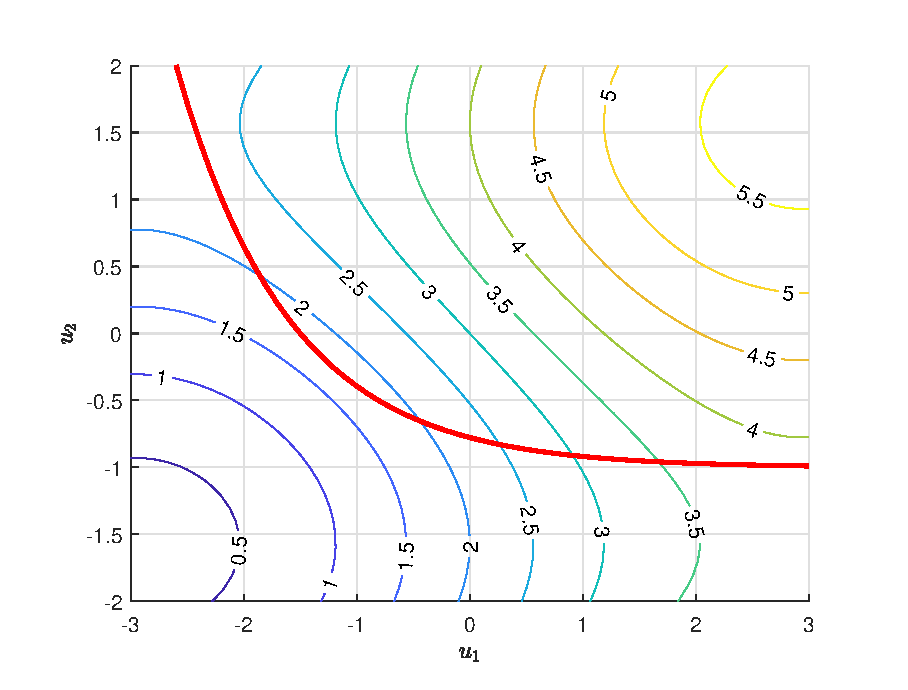
\includegraphics[width=300pt]{chapters/ch-optimal-robust-control-system/figures/opt_equalityconstraint_contour.eps}
	\caption{Static optimization with equality constraint demonstration.} \label{fig:optimalrobustcs:opt_equalityconstraint_contour}
\end{figure}
where $L(u)$ is given by the contour (assuming $u\in\mathbb{R}^2$ in this demonstration), and $f(u)=0$ the red solid line.

The critical point of \eqref{eq:optimalrobustcs:equalityconsfunc} can be found as follows. Consider a necessary condition for the critical point. At the critical point, $L_u = dL / du$ is not necessary zero, and neither is $dL$ for all random chosen $du$. However, $dL$ should be zero with respect to $du$ when $df$ is zero, i.e. (consider only the first-order Taylor expansion for now),
\begin{eqnarray}
	&& dL = L_u^Tdu = 0 \label{eq:optimalrobustcs:equalitycritical1} \\
	\textit{s.t.} && df = f_udu = 0 \label{eq:optimalrobustcs:equalitycritical2}
\end{eqnarray}
or equivalently
\begin{eqnarray}
	\left[\begin{array}{c}
		dL_{\color{red} 1\times 1} \\ df_{\color{red} n\times 1}
	\end{array}\right]_{\color{red} (n+1)\times 1} = \left[\begin{array}{c}
	{L_u^T}_{\color{red} 1\times m} \\ {f_u}_{\color{red} n\times m}
	\end{array}\right]_{\color{red} (n+1)\times m}du_{\color{red} m\times 1} = 0 \label{eq:optimalrobustcs:equalitycritical3}
\end{eqnarray}
For reading convenience, the dimensions of the matrices are given in red color.

As a necessary condition, given a critical point, we should be able to solve \eqref{eq:optimalrobustcs:equalitycritical2} for a linear space of $du$, and make sure that such $du$ satisfies \eqref{eq:optimalrobustcs:equalitycritical1}. With that been said, the coefficient matrix $[L_u^T; f_u]$ in \eqref{eq:optimalrobustcs:equalitycritical3} should have rank of at most $n$ so that the last $n$ rows alone can be used to find $du$ then substitute it to the first row for verification. Therefore, \eqref{eq:optimalrobustcs:equalitycritical3} can be re-written as follows.
\begin{eqnarray}
	\left[\begin{array}{cc}
		1 & \lambda^T
	\end{array}\right] \left[\begin{array}{c}
	L_u^T \\ f_u
	\end{array}\right] &=& 0 \nonumber \\
	L_u^T + \lambda^Tf_u &=& 0 \label{eq:optimalrobustcs:equalitycritical4}
\end{eqnarray}
where $\lambda \in \mathbb{R}^n$ is known as the Lagrange multipliers, and \eqref{eq:optimalrobustcs:equalitycritical4} a set of $m$ equations being a simplified part of Karush–Kuhn–Tucker (KKT) conditions which will be introduced in more details later.

Equation \eqref{eq:optimalrobustcs:equalitycritical4} can also be interpreted graphically. It suggest that the gradient of $L(u)$ and $f(u)$ should be parallel at the critical point by a factor of $\lambda$. This is shown by Fig. \ref{fig:optimalrobustcs:opt_equalityconstraint_graphical}. At the critical point denoted by the red dot, the red solid line $f(u)=0$ tangents the contour $L(u)$ indicated by the red dashed line. The gradient of both $f_u=\nabla f$ and $L_u=\nabla L$ should be perpendicular to the tangent aligning with the red arrows, hence they are parallel.
\begin{figure}
	\centering
	\includegraphics[width=300pt]{chapters/ch-optimal-robust-control-system/figures/opt_equalityconstraint_graphical.png}
	\caption{Graphical explanation to \eqref{eq:optimalrobustcs:equalitycritical4}.} \label{fig:optimalrobustcs:opt_equalityconstraint_graphical}
\end{figure}

Equation \eqref{eq:optimalrobustcs:equalitycritical4} together with \eqref{eq:optimalrobustcs:equalityconstraint} forms the necessary condition for the solution of the optimization problem.

\vspace{0.1in}
\noindent \textbf{Lagrangian Function}
\vspace{0.1in}

The necessary condition can also be derived using Lagrangian function as follows. Lagrangian function is a very useful tool in solving optimization problem with different types of constraints. Notice that Lagrangian function in some context may also be called Hamiltonian function. They are very similar mathematically, and mostly differ in the context of usage.
\begin{eqnarray}
	\mathcal{L}(u, \lambda) &=& L(u) + \lambda^Tf(u) \label{eq:optimalrobustcs:lagarangianequality} \\
	&=& L(u) + \sum_{i=1}^{n}\lambda_if_i(u) \nonumber
\end{eqnarray}
and \eqref{eq:optimalrobustcs:equalityconstraint}, \eqref{eq:optimalrobustcs:equalitycritical4} can be represented by
\begin{eqnarray}
	\dfrac{\partial \mathcal{L}}{\partial \lambda} &=& 0 \nonumber \\
	\dfrac{\partial \mathcal{L}}{\partial u} &=& 0 \nonumber
\end{eqnarray}
respectively.

It is difficult to find the critical point for the original problem with equality constraint. However, by introducing Lagrangian function \eqref{eq:optimalrobustcs:lagarangianequality}, the problem becomes finding critical point for Lagrangian function without constraint (by considering both $\lambda$ and $u$ as the independent variable of $\mathcal{L}$). The converted problem, which is simpler to solve, is known as the dual problem of the original problem. This is made possible due to the introduction of Lagrange multipliers $\lambda$ that adds some flexibility to the equation, making it contain the information of equality constraint in a ``disguised'' manner.

\vspace{0.1in}
\noindent \textbf{Sufficient Condition}
\vspace{0.1in}

The necessary condition helps to pick up the possible candidates that may be a local minimum of the optimization problem. To verify that the critical point is indeed a local minimum, check the second-order derivative $\partial^2 L / \partial u^2$ of the critical point.

Consider the following example.
\begin{shortbox}
\Boxhead{A Quadratic Surface Example with Linear Equality Constraint}

Let
\begin{eqnarray}
	&& L(x, u) = \dfrac{1}{2}x^TQx + \dfrac{1}{2}u^TRu \label{eq:optimalrobustcs:quadraticsurfexp1} \\
	\textup{s.t.} && f(x, u) = x + Bu + c = 0 \nonumber
\end{eqnarray}
where the dimensions are $x\in\mathbb{R}^n$, $u\in\mathbb{R}^m$, $Q\in\mathbb{R}^{n\times n}$, $R\in\mathbb{R}^{m\times m}$, $B\in\mathbb{R}^{n\times m}$, $c\in\mathbb{R}^n$. Find $u$ at the critical point, and discuss whether it is a minimum.

\end{shortbox}

The Lagrangian function of the problem is
\begin{eqnarray}
  \mathcal{L} &=& \dfrac{1}{2}x^TQx + \dfrac{1}{2}u^TRu + \lambda^T(x + Bu + c) \nonumber
\end{eqnarray}
where $\lambda \in\mathbb{R}^n$. The necessary condition for a critical point is
\begin{eqnarray}
  \dfrac{\partial \mathcal{L}}{\partial \lambda} &=& x + Bu + c = 0 \\
  \dfrac{\partial \mathcal{L}}{\partial x} &=& Qx + \lambda = 0 \\
  \dfrac{\partial \mathcal{L}}{\partial u} &=& Ru + B^T\lambda = 0 \nonumber
\end{eqnarray}
The solution is
\begin{eqnarray}
  u &=& -\left(R+B^TQB\right)^{-1}B^TQc \label{eq:optimalrobustcs:quadraticsurfexp2} \\
  x &=& -\left(I-B\left(R+B^TQB\right)^{-1}B^TQ\right)c \label{eq:optimalrobustcs:quadraticsurfexp3} \\
  \lambda &=& \left(Q^{-1}+BR^{-1}B^T\right)^{-1}c \nonumber
\end{eqnarray}
The verify whether it is a minimum w.r.t. $u$, check the following
\begin{eqnarray}
  L_{uu} &=& R+B^TQB \nonumber
\end{eqnarray}
which is positive definite as long as $Q$ and $R$ are positive definite. Indeed, this is a minimum w.r.t. $u$. The minimum value can be obtained by substituting \eqref{eq:optimalrobustcs:quadraticsurfexp2} and \eqref{eq:optimalrobustcs:quadraticsurfexp3} into \eqref{eq:optimalrobustcs:quadraticsurfexp1}.
\begin{eqnarray}
  L^* &=& \dfrac{1}{2}c^T\left(Q^{-1}+BR^{-1}B^T\right)^{-1}c \nonumber \\
  &=& \dfrac{1}{2}c^T\lambda \nonumber
\end{eqnarray}

\subsection{Optimization with Equality and Inequality Constraints}

Optimization with inequality constraints is not as widely seen in optimal control as optimization with equality constraint. Nevertheless, it is briefly introduced here. Consider the optimization problem with both equality and inequality constraints as follows.
\begin{eqnarray}
	\textup{minimize} && L(u) \nonumber \\
	\textup{s.t.} && f(u) = 0 \nonumber \\
    && g(n) \leq 0 \label{eq:optimalrobustcs:inequalityconstraint2}
\end{eqnarray}
where $u\in\mathbb{R}^m$, $f(u)\in\mathbb{R}^p$, $g(u)\in\mathbb{R}^q$.

Obviously, the solution of the problem may reside at either $g(u)=0$ or $g(u)<0$. Therefore, an intuitive way of solving the problem is to use ``trail-and-error'' as follows. Ignore the inequality constraint \eqref{eq:optimalrobustcs:inequalityconstraint2}, and the problem becomes an optimization with equality constraint problem. Test the obtained solution using \eqref{eq:optimalrobustcs:inequalityconstraint2}. If \eqref{eq:optimalrobustcs:inequalityconstraint2} is satisfied, the solution to the new problem is also a solution to the original problem. Otherwise, reformulate the problem and let both $f(u)=0$, $g(u)=0$ be equality constraints.

Sort of inspired by this idea, the optimization problem with both equality and inequality constraints described by \eqref{eq:optimalrobustcs:inequalityconsfunc}, \eqref{eq:optimalrobustcs:inequalityconstraint1} and \eqref{eq:optimalrobustcs:inequalityconstraint2} can be solved as follows. First, define generalized Lagrangian function
\begin{eqnarray}
  \mathcal{L}(u, \alpha, \beta) &=& L(u) + \alpha^Tf(u) + \beta^Tg(u) \nonumber
\end{eqnarray}
where $\alpha\in\mathbb{R}^p$ and $\beta\in\mathbb{R}^q$ are Lagrange multipliers associated with equality and inequality constraints, respectively. In some literatures, $\lambda = \left[\begin{array}{cc}
        \alpha^T & \beta^T
      \end{array} \right]^T$ might be used in the notation.

The necessary condition for a solution can be obtained using Karush-Kuhn-Tucker (KKT) conditions as follows. The KKT conditions are essentially first derivative tests for the solution to be optimal. Notice that sometimes KKT can be necessary and sufficient condition for the solution if $L$, $f$ and $g$ meet certain criteria. This is not discussed here in details.
\begin{eqnarray}
  \dfrac{\partial \mathcal{L}}{\partial u} &=& 0 \label{eq:optimalrobustcs:kkt1} \\
  \dfrac{\partial \mathcal{L}}{\partial \alpha} &=& 0 \label{eq:optimalrobustcs:kkt2} \\
  \beta_i g_i(u) &=& 0 \label{eq:optimalrobustcs:kkt3} \\
  g_i(u) &\leq& 0 \label{eq:optimalrobustcs:kkt4} \\
  \beta_i &\geq& 0 \label{eq:optimalrobustcs:kkt5}
\end{eqnarray}
Equations \eqref{eq:optimalrobustcs:kkt1} and \eqref{eq:optimalrobustcs:kkt2} are straight forward and they are the same with the previous discussed optimization with equality constraint problem. Equations \eqref{eq:optimalrobustcs:kkt3}, \eqref{eq:optimalrobustcs:kkt4} and \eqref{eq:optimalrobustcs:kkt5} discusses how the inequality constraint would affect the critical point:
\begin{itemize}
  \item In Lagrangian function, let the inequality constraint does not affect its value, hence \eqref{eq:optimalrobustcs:kkt3}.
  \item Equation \eqref{eq:optimalrobustcs:kkt3} is achieved as follows:
  \begin{itemize}
    \item If the critical point is laid on the $i$th inequality constraint boundary, $g_i(u)=0$, making \eqref{eq:optimalrobustcs:kkt3} zero. In this case, the value of $\beta_i$ does not matter. Without loosing generality, let $\beta_i>0$.
    \item If the critical point is not laid on the $i$th inequality constraint boundary, $g_i(u)<0$, in which case enforce $\beta_i=0$ so that \eqref{eq:optimalrobustcs:kkt3} is zero.
    \item In other words, if $g_i(u)<0$, $\beta_i=0$; if $g_i(u)=0$, $\beta_i>0$.
  \end{itemize}
\end{itemize}

Equations \eqref{eq:optimalrobustcs:kkt1} to \eqref{eq:optimalrobustcs:kkt5} together form the dual problem of the original problem. Equation \eqref{eq:optimalrobustcs:kkt3} is known as the complementary slackness, and \eqref{eq:optimalrobustcs:kkt5} dual feasibility.

\section{Optimal Control of Discrete System} \label{sec:optimalrobustcs:discrete}

Optimal control system has a strong connection with the static optimization problem introduced in Section \ref{sec:optimalrobustcs:static}. In mathematics perspective, they are using similar tools to solve similar problems. It is just that the physical model of the system, which determines how the system evolves giving a control signal, becomes the constraint in the optimization. This is illustrated in the remaining of the chapter.

\subsection{Problem Formulation}

A general optimal control of discrete system problem can be described as follows. Let the system dynamics be described by
\begin{eqnarray}
  x(k+1) &=& f^k\left(x(k), u(k)\right) \label{eq:optimalrobustcs:generaldynamic}
\end{eqnarray}
where $k=0,\ldots$ is the time index, $x(k)\in\mathbb{R}^n$ the state vector ($x(0)$ is the initial state), $u(k)\in\mathbb{R}^m$ the input and $f^k$ the system dynamics. No disturbance or process error is considered. It is assumed that $x(k)$ is known at all time instant.

The objective of the optimization is to find such $u(k)$ that minimizes the following cost function
\begin{eqnarray}
  J &=& \phi\left(N, x(N)\right) + \sum_{k=0}^{N-1}L^k\left(x(k), u(k)\right) \label{eq:optimalrobustcs:generaldiscrete}
\end{eqnarray}
where $N$ is the time to reach a particular goal, $x(N)$ the final state vector at $k=N$, and $L^k$ the cost relevant to the magnitude of $x(k)$ and $u(k)$ at time instant $k$. In some cases, $N$ is a parameter to optimize, for example in a ``do-it-fast'' type of problem. In other cases, $N$ is a fixed value, for example in a ``do-the-best-within-given-time'' type of problem.

Some commonly seen cost functions are given below.

\vspace{0.1in}
\noindent \textbf{Minimum Time}
\vspace{0.1in}

Use $u(k)$ to drive the system from its initial state to a given state. The total time consumption is minimized.
\begin{eqnarray}
  J &=& N \nonumber
\end{eqnarray}

\vspace{0.1in}
\noindent \textbf{Minimum Fuel and Energy}
\vspace{0.1in}

Use $u(k)$ to drive the system from its initial state to a given state. The cost of applying the control signal is minimized. To minimize the fuel consumption,
\begin{eqnarray}
  J &=& \sum_{k=0}^{N-1} |u(k)| \nonumber
\end{eqnarray}
To minimize energy,
\begin{eqnarray}
  J &=& \sum_{k=0}^{N-1} u(k)^Tu(k) \nonumber
\end{eqnarray}

\vspace{0.1in}
\noindent \textbf{Regulation}
\vspace{0.1in}

Use $u(k)$ to regulate the states to zero (usually from a non-zero initial state). Along the way, both regulation error and the control signal driving energy are considered.
\begin{eqnarray}
  J &=& \dfrac{1}{2}x(N)^TSx(N) + \dfrac{1}{2}\sum_{k=0}^{N-1}\left(x(k)^TQx(k) + u(k)^TRu(k)\right) \nonumber
\end{eqnarray}
where $Q$, $S$ and $R$ are weight matrices that trades of the minimization of regulation error (intermediate state error), final state error or control signal energy.

\subsection{General Solution} \label{subsec:optimalrobustcs:optimalgeneralsolution}

A general solution to \eqref{eq:optimalrobustcs:generaldiscrete} subject to \eqref{eq:optimalrobustcs:generaldynamic} is given below.

Define the augmented cost function as the Lagrangian function below, taking into account \eqref{eq:optimalrobustcs:generaldynamic} as the equality constraint.
\begin{eqnarray}
	J\textprime &=& \phi\left(N, x(N)\right) + \sum_{k=0}^{N-1}\left(L^k\left(x(k), u(k)\right) + \lambda_{k+1}^T\left(f^k\left(x(k), u(k)\right) - x(k+1)\right)\right) \nonumber
\end{eqnarray}
which can be rewritten as
\begin{eqnarray}
	J\textprime &=& \phi\left(N, x(N)\right) - \lambda_N^Tx(N) + H^0(x(0), u(0)) \nonumber \\
	&& + \sum_{k=0}^{N-1}\left(H^k\left(x(k), u(k)\right) - \lambda_k^Tx(k)\right) \nonumber
\end{eqnarray}
where
\begin{eqnarray}
	H^k\left(x(k), u(k)\right) &=& L^k\left(x(k), u(k)\right) + \lambda_{k+1}^Tf^k\left(x(k), u(k)\right) \nonumber
\end{eqnarray}
is the Hamiltonian defined at each time stamp $k$. Apply KKT condition and the solution is
\begin{eqnarray}
	x(k+1) &=& \dfrac{\partial H^k}{\partial \lambda_{k+1}} = f^k\left(x(k), u(k)\right) \nonumber \\
	\lambda_k &=& \dfrac{\partial H^k}{\partial x(k)} = \left(\dfrac{\partial f^k}{\partial x(k)}\right)^T\lambda_{k+1} + \dfrac{\partial L^k}{\partial x(k)} \nonumber \\
	0 &=& \dfrac{\partial H^k}{\partial u(k)} = \left(\dfrac{\partial f^k}{\partial u(k)}\right)^T\lambda_{k+1} + \dfrac{\partial L^k}{\partial u(k)} \nonumber \\
	0 &=& \left(\dfrac{\partial L^0}{\partial x(0)} + \left(\dfrac{\partial f^0}{\partial x(0)}\right)^T\lambda_1\right)^Tdx(0) \nonumber \\
	0 &=& \left(\dfrac{\partial \phi}{\partial x(N)}-\lambda_N\right)^Tdx(N) \nonumber
\end{eqnarray}

\subsection{Discrete LQR}

Linear quadratic regulator (LQR) is a special case of the general problem formulation \eqref{eq:optimalrobustcs:generaldynamic} and \eqref{eq:optimalrobustcs:generaldiscrete}. It is one of the most commonly seen optimal control problems.

Consider linear system as follows. It is assumed that the state vector is known exactly.
\begin{eqnarray}
	x(k+1) &=& A(k)x(k) + B(k)u(k) \nonumber
\end{eqnarray}
where notice that the process matrix $A(k)$, input matrix $B(k)$ can be time-varying. The cost function is given by
\begin{eqnarray}
	J &=& \dfrac{1}{2}x(N)^TS_Nx(N) + \dfrac{1}{2}\sum_{k=0}^{N-1}\left(x(k)^TQ_kx(k) + u(k)^TR_ku(k)\right) \nonumber
\end{eqnarray}
where $|S_N|\geq 0$, $|Q_k| \geq 0$ and $|R_k| >0$ are known symmetric matrices. In the LQR problem, the target of the control is to regulate the state vector to zero while given an non-zero initial state, and meantime tries to keep the control signal energy small.

The solution of the problem can be found by constructing the Hamiltonian function as introduced earlier in Section \ref{subsec:optimalrobustcs:optimalgeneralsolution}. Result is given below.
\begin{eqnarray}
	S_k &=& A(k)^T\left(S_{k+1}-S_{k+1}B(k)\left(B(k)^TS_{k+1}B(k) + R_k\right)^{-1}B(k)^TS_{k+1}\right)A(k)  \nonumber \\ && + Q_k \label{eq:optimalrobustcs:srecursive} \\
	K(k) &=& \left(B(k)^TS_{k+1}B(k) + R_k\right)^{-1}B(k)^TS_{k+1}A(k) \label{eq:optimalrobustcs:lqrkalman} \\
	u(k) &=& -K(k)x(k) \nonumber
\end{eqnarray}
where $k=0,\ldots, N-1$. Matrix $K(k)$ in \eqref{eq:optimalrobustcs:lqrkalman} is known as the Kalman gain (it might be more intuitive to simply call it the ``control gain'') and it can be calculated offline.

\subsection{Suboptimal Discrete LQR} \label{subsec:suboptimaldiscretelqr}

Notice that $K(k)$ is time varying in general. Only if $A$, $B$, $Q$ and $R$ are constant and at the same time $N\rightarrow\infty$, $S_k$ becomes a constant and so does $K(k)$. In such case, the cost function becomes
\begin{eqnarray}
	J &=& \dfrac{1}{2}\sum_{k=0}^{\infty}\left(x(k)^TQx(k) + u(k)^TRu(k)\right) \nonumber
\end{eqnarray}

The problem can be solved similarly with $S$ the unique positive definite solution to the following discrete time algebraic Riccati equation
\begin{eqnarray}
	S &=&  A^T\left(S-SB\left(B^TSB + R\right)^{-1}B^TS\right)A \label{eq:optimalrobustcs:sstatics}
\end{eqnarray}
and the Kalman gain
\begin{eqnarray}
	K_\infty &=& \left(B^TSB + R\right)^{-1}B^TSA \label{eq:optimalrobustcs:statickalmangain}
\end{eqnarray}
which is also known as the static Kalman gain.

In a LTI system where $A$, $B$, $Q$ and $R$ are constant matrices and $N$ a finite number, dealing with time varying $K(k)$ can be problematic in practice due to the large memory and offline computation load requirement. It is sometimes preferable to rather use suboptimal control $u=-K_\infty x(k)$ instead of $u=-K(k)x(k)$, where $K_\infty$ is calculated using \eqref{eq:optimalrobustcs:statickalmangain}, assuming $N\rightarrow\infty$ and ignoring $x(N)^TS_Nx(N)$ in the cost function.

It is important to verify whether the system remains asymptotically stable when suboptimal control law is applied. Only the conclusion is given as follows: the system $(A,B)$ is stabilizable if and only if:
\begin{itemize}
	\item Equation \eqref{eq:optimalrobustcs:sstatics} has unique positive definite solution, and \eqref{eq:optimalrobustcs:srecursive} converges to that solution.
	\item The closed-loop plant $(A-BK_\infty)$ is asymptotically stable.
\end{itemize}
The proof is ignored.

This implies that so long as the original system is stabilizable, the suboptimal control $u=-K_\infty x(k)$ guarantees the asymptotic stability of the system.

\section{Optimal Control of Continuous System}

The dynamics of a continuous time domain system is described using differential equations, and the solution can be obtained using Lagrangian function similar to previous sections. However, do notice that calculus of variations is used when solving the problem. Calculus of variations is briefly reviewed in the appendix. For more details of calculus of variations, check \textit{A Notebook on Calculus} by Lu Sun in the same series.

\subsection{Problem Formulation}

Let the system dynamics be described by the following state-space model
\begin{eqnarray}
	\dot{x} &=& f(x, u, t) \nonumber
\end{eqnarray}
where $x(t)\in \mathbb{R}^n$, $u(t)\in\mathbb{R}^m$. Let the cost function be
\begin{eqnarray}
	J &=& \phi\left(x(T), T\right) + \int_{0}^{T} L\left(x(t), u(t), t\right)dt \label{eq:optimalrobustcs:jcontinuouslqr}
\end{eqnarray}
where $[0, T]$ is the time interval of interest. The final time $T$ may vary when different controls are applied. In addition, define $\psi\left(x(T), T\right)$. The objective of the optimization is to find optimal $u(t)$ on the time interval $[0, T]$, so that $J$ in \eqref{eq:optimalrobustcs:jcontinuouslqr} is minimized, and $\psi\left(x(T), T\right) = 0$.

Notice that $\psi$ is different from $\phi$ in \eqref{eq:optimalrobustcs:jcontinuouslqr}. Both of them are about the final state, but $\phi$ is made small while $\psi$ needs to be made exactly zero. This restriction introduced by $psi$ is useful. For example, in a position regulation problem, $\psi$ can be defined as
\begin{eqnarray}
	\psi &=& \left[\begin{array}{c}
		x(T) - X \\ \dot{x}(T)
	\end{array}\right] \nonumber
\end{eqnarray}
where $x(T) - X=0$ enforces zero regulation error, and $\dot{x}(T)=0$ enforces a complete stop of the system motion.

\subsection{General Solution}

Define the augmented cost function as the Lagrangian function below.
\begin{eqnarray}
	J\textprime &=& \phi\left(x(T),T\right) + \nu^T\psi\left(x(T),T\right) \nonumber \\
	&& + \int_{0}^{T}\left(L(x, u, t) + \lambda^T\left(f(x, u, t) - \dot{x}\right)\right)dt \nonumber
\end{eqnarray}
where $\nu$, $\lambda$ are Lagrange multipliers. Define Hamiltonian function as follows.
\begin{eqnarray}
	H(x,u,t) &=& L(x, u, t) + \lambda^Tf(x, u, t) \nonumber
\end{eqnarray}
The solution of the optimization problem can be obtained by letting
\begin{eqnarray}
	\begin{array}{cc}
		\textup{State:} & \dot{x} = \dfrac{\partial H}{\partial \lambda} = f \\ & \\
		\textup{Costate:} & -\dot{\lambda} = \dfrac{\partial H}{\partial x} = \dfrac{\partial f^T}{\partial x}\lambda + \dfrac{\partial L}{\partial x} \\ & \\
		\textup{Stationarity:} & 0 = \dfrac{\partial H}{\partial u} = \dfrac{\partial L}{\partial u} + \dfrac{\partial f^T}{\partial u}\lambda \\ & \\
		\textup{Boundary:} & x(0)\textup{~is given} \\ & \\
		& \left.\left(\phi_x+\psi_x^T\nu-\lambda\right)^T\right|_{T}dx(T) + \left.\left(\phi_t+\psi_t^T\nu+H\right)^T\right|_{T}dT = 0
	\end{array} \nonumber
\end{eqnarray}

It is often not easy to solve analytical solution of $u(t)$ from the above equations.

\subsection{Continuous LQR}

LQR in discrete time domain has been introduced earlier. Its application in continuous time domain is introduced in this section as follows. Let the system dynamics be described by
\begin{eqnarray}
	\dot{x}(t) = A(t)x(t) + B(t)u(t) \nonumber
\end{eqnarray}
where $x(t)\in\mathbb{R}^n$ and $u(t)\in\mathbb{R}^m$. The state vector $x(t)$ is assumed known exactly. The cost function is given by
\begin{eqnarray}
  J &=& \dfrac{1}{2}x(T)^TS_Tx(T) + \dfrac{1}{2}\int_{0}^{T}\left(x(t)^TQ_tx(t) + u(t)^TR_tu(t)\right)dt \nonumber
\end{eqnarray}
where $|S_T|\geq 0$, $|Q_t| \geq 0$ and $|R_t| >0$ are known symmetric matrices.

The solution can be obtained by formulating the Hamiltonian. Result is given below.
\begin{eqnarray}
  -\dot{S}(t) &=& A(t)^TS(t) + S(t)A(t) - S(t)B(t)R_t^{-1}B(t)^TS(t) + Q_t \label{eq:optimalrobustcs:csrecursive} \\
  K(t) &=& R_t^{-1}B(t)^TS(t) \label{eq:optimalrobustcs:lqrckalman} \\
  u(t) &=& -K(t)x(t) \nonumber 
\end{eqnarray}

\subsection{Suboptimal Continuous LQR}

Just like Section \ref{subsec:suboptimaldiscretelqr}, the continuous LQR also has suboptimal solution. The motivation remains the same: to tackle the problem where Kalman gain $K(t)$ in \eqref{eq:optimalrobustcs:lqrckalman} is time-varying and can be difficult or tedious to calculate, and we want an alternative solution with constant Kalman gain.

Assume time-invariant $A$, $B$ in the process model and constant $Q$, $R$. Let time-invariant $S$ be the solution of the following ARE
\begin{eqnarray}
	0 &=& A^TS + SA - SBR^{-1}B^TS + Q \label{eq:optimalrobustcs:sare}
\end{eqnarray}
which is obtained from \eqref{eq:optimalrobustcs:csrecursive} by letting $\dot{S}=0$ assuming convergence. Notice that the solution to \eqref{eq:optimalrobustcs:sare} is not necessarily unique. One of the solutions of $S$ can be obtained by calculating \eqref{eq:optimalrobustcs:csrecursive} until it converges to $S(\infty)$, and $S=S(\infty)$ is obviously a solution to \eqref{eq:optimalrobustcs:sare}. This would be the solution that we would use through out the remaining of the section. Alternatively, $S$ can be calculated using the analytical solution to the ARE which is not covered in this notebook.

With the obtained constant $S=S(\infty)$, Kalman gain in \eqref{eq:optimalrobustcs:lqrckalman} becomes
\begin{eqnarray}
	K &=& R^{-1}B^TS(\infty) \nonumber
\end{eqnarray}
which is time-invariant. This produces a suboptimal solution but with a constant Kalman gain that is easier for implementation.

\section{LQR Properties}

The problem formulation and the solution of LQR have been introduced in earlier sections. The properties, extensions, practical implementations, etc., have not yet been covered. In this section and the few sections following, these more advanced topics are discussed.

In this section, we will start with the discussion of LQR properties, such as its robustness.

\section{LQR for Tracking Problem}

LQR by itself is a regulator that regulates the state vector $x$ to a constant value $r$, and at the same time balancing the control signal energy. LQR can also be used in tracking, in which case the reference signal is no longer a constant, but time-variant. Tracking is an important extension of LQR.

 















\section{Other LQR Extensions}






























 

\section{LQG}

\section{$H_2$ and $H_\infty$ Control} 